\documentclass[12pt]{article}
\usepackage{amsmath, amssymb,graphicx, natbib, setspace, times}
\usepackage[usenames]{color}
\usepackage{fullpage}
\definecolor{DarkRed2}{rgb}{0.6,0,0.08}
\newcommand{\indep}{{\;\bot\!\!\!\!\!\!\bot\;}}

\title{\texttt{eiPack}: Tools for R $\times$ C Ecological
Inference and Higher-Dimension Data Management}

\author{Olivia Lau \and Ryan T. Moore \and Michael
Kellermann\footnote{\texttt{olau@fas.harvard.edu},
\texttt{rtmoore@fas.harvard.edu}, and
\texttt{kellerm@fas.harvard.edu}.  Department of Government and Institute for Quantitative Social Science, Harvard University, 1737
Cambridge Street, Cambridge MA 02138}}

\begin{document}
\maketitle

\section{Introduction}

Under certain conditions, ecological inference ({\sc ei}) models allow
researchers to infer individual-level behavior from aggregate data
when individual-level data is unavailable.  Table \ref{t:ei} shows a
typical unit of ecological analysis: a contingency table with observed
row and column marginals and unobserved interior cells.

\begin{table}[h!]
\begin{center}
\begin{tabular}{l|ccc|c}
	& $\rm{col}_1$ & $\rm{col}_2$ & $\rm{col}_3$ & \\
\hline
$\rm{row}_1\quad$	& \color{DarkRed2}{$\quad N_{11i}\quad$} &
\color{DarkRed2}{$\quad N_{12i}\quad$} &
\color{DarkRed2}{$\quad N_{13i}\quad$} & $\quad N_{1\cdot i}$ \\
$\rm{row}_2\quad$ 	& \color{DarkRed2}{$N_{21i}$} & \color{DarkRed2}{$N_{22i}$} &
\color{DarkRed2}{$N_{23i}$} & $\quad N_{2\cdot i}$ \\ 
$\rm{row}_3\quad$	& \color{DarkRed2}{$N_{31i}$} & \color{DarkRed2}{$N_{32i}$} &
\color{DarkRed2}{$N_{33i}$} & $\quad N_{3\cdot i}$ \\ 
\hline
	& $N_{\cdot 1i}$ & $N_{\cdot 2i}$ & $N_{\cdot 3i}$ & $\quad N_i$
\end{tabular} 
\end{center}
\caption{A typical $R \times C$ unit in ecological inference;
\color{DarkRed2}{red} quantities are typically unobserved.}
\label{t:ei}
\end{table}

Existing packages that implement {\sc ei} methods, such as
\texttt{eco} and \texttt{MCMCpack}, focus on $2 \times 2$
inference. \texttt{eiPack} offers methods for the more general case in
which the ecological units are $R \times C$ tables.  

\section{Methods and Data in \texttt{eiPack}}

The methods currently implemented in \texttt{eiPack} are the method of
bounds \citep{DunDav53}, ecological regression \citep{Goodman53}, and
the Multinomial-Dirichlet model \citep{RosJiaKin01}.

The functions that implement these models share
several attributes.  The ecological tables are defined using a
common formula of the form \texttt{cbind(col1, ..., colC)} $\sim$
\texttt{cbind(row1, ...,rowR)}.  The row and column marginals can be
expressed as either proportions or counts.  Auxiliary functions
renormalize the results for some subset of columns taken from the
original ecological table, and appropriate \texttt{print},
\texttt{summary}, and \texttt{plot} functions conveniently summarize
the model output.

In the following section, we demonstrate the features of
\texttt{eiPack} using the (included) \texttt{senc} dataset, which
contains individual-level party affiliation data for Black, White, and
Native American voters in 8 counties in southeastern North Carolina.
These counties include 212 precincts, which form the ecological units
in this dataset.  Because the data are observed at the individual
level, the interior cell counts are known, allowing us to benchmark
the estimates implied by each method.

\subsection{Method of Bounds}

The method of bounds \citep{DunDav53} uses the observed row and column
marginals to calculate deterministic upper and lower bounds for
functions of the interior cells of each ecological unit.  As
implemented in \texttt{eiPack}, it calculates for a specified column $k'
\in k = \{1, \dots, C\}$ the deterministic bounds on the proportion of
individuals in each row who belong in that column.  For each
unit being considered, let $j$ be the row of interest, $k$ index
columns, $k'$ be the column of interest, $k''$ be the set of other
columns considered, and $\tilde{k}$ be the set of columns excluded.
For example, if we want the bounds on the proportion of Native
American two-party registrants who are Democrats, $j$ is Native
American, $k'$ is Democrat, $k''$ is Republican, and $\tilde{k}$ is No
Party.  The unit-level quantity of interest is

\begin{displaymath}
\frac{N_{jk'i}}{N_{jk'i} + \sum_{k \in k''} N_{jki}}
\end{displaymath}

\noindent The lower and upper bounds on this quantity given by the
observed marginals are, respectively:

\begin{displaymath}
\frac{\max(0, N_{ji} - \sum_{k \neq k'} N_{ki})}{\max(0, N_{ji} - \sum_{k \neq
k'} N_{ki}) + \min(N_{ji}, \sum_{k \in k''} N_{ki})}
\end{displaymath}

\noindent and

\begin{displaymath}
\frac{\min(N_{ji}, N_{k'i})}{\min(N_{ji}, N_{k'i}) + \max(0, N_{ji} - N_{k'i} - \sum_{k \in \tilde{k}} N_{ki})}
\end{displaymath}

The method of bounds is not a statistical procedure in the traditional
sense; the bounds implied by the row and column marginals are
deterministic and there is no model of the data-generating
process. One population-level quantity of interest calculated by
\texttt{eiPack} is the interval defined by the intersection of the
unit-level bounds \citep{Grofman00}.  This interval, if it exists,
represents the range of values that are consistent with the observed
marginals in all of the ecological units.

Since the bounds become more informative as within-unit homogeneity increases, researchers and
practitioners often restrict their attention to those units in which
one group dominates.  \texttt{eiPack} allows users to set row
thresholds to conduct this
\textit{extreme case analysis} (also known as  \textit{homogeneous
precinct analysis} in the voting context).
For example, suppose the user is interested in the proportion of
two-party White registrants registered as Democrats in precincts that
are at least 90\% White.  \texttt{eiPack} calculates the desired bounds:
\begin{verbatim}
> out <- bounds(cbind(dem, rep, non) ~ cbind(black, white, natam),
+   data = senc, rows = c("white"), column = "dem", 
+   excluded = "non", threshold = 0.9, total = NULL)
\end{verbatim} %$
These calculated bounds can then be represented graphically; in this
example, there is no interval consistent with the bounds in each
precinct:
\begin{verbatim}
> plot(out, row = "white", column = "dem")
\end{verbatim}
\begin{figure}[h!]
\begin{center}
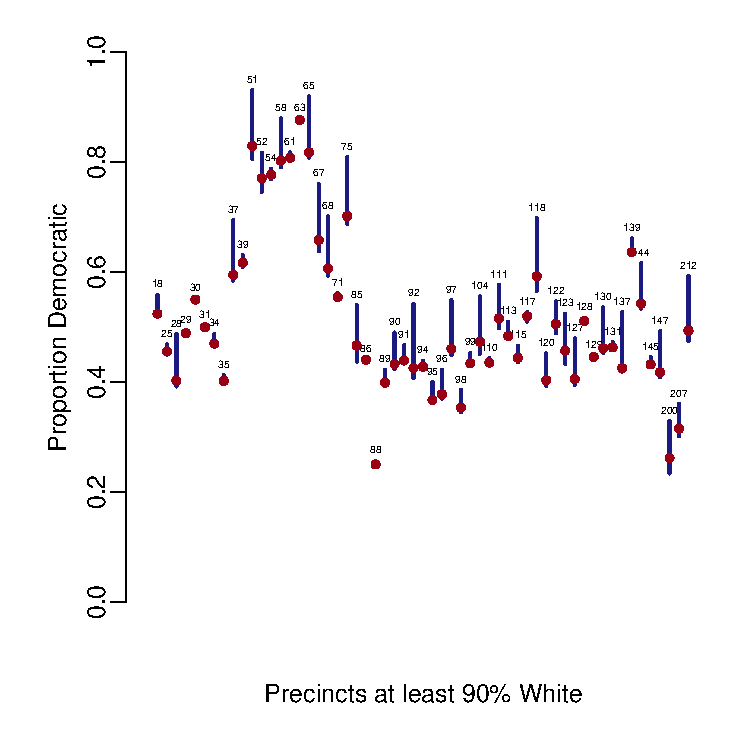
\includegraphics[height=3.2in]{white.pdf}
\end{center}
\caption{A plot of deterministic bounds.}
\label{f:mob} 
\end{figure}

\subsection{Ecological Regression}

In ecological regression \citep{Goodman53}, observed row and column
marginals are expressed as proportions and each column is regressed
separately on the row proportions, thus performing $C$ regressions.  
Regression coefficients then estimate the population internal cell
proportions.  For a given unit $i$, define

\begin{itemize}
\item $X_{ri}$, the proportion of individuals in row $r$,
\item $T_{ci}$, the proportion of individuals in column $c$, and
\item $\beta_{rci}$, the proportion of row $r$ individuals in column
$c$
\end{itemize}

\noindent The following identities hold:
\begin{displaymath}
T_{ci} \; = \; \sum_{r=1}^R \beta_{rci} X_{ri} \quad \textrm{and} \quad \sum_{c=1}^{C} \beta_{rci}  \; = \; 1    
\end{displaymath}
\noindent  Defining the population cell fractions $\beta_{rc}$ such that
$\sum_{c=1}^C \beta_{rc} = 1$ for every $r$, ecological regression assumes that
$\beta_{rc} = \beta_{rci}$ for all $i$, and estimates the regression
equations $T_{ci} = \beta_{rc} X_{ri} + \epsilon_{ci}$.  Under the
standard linear regression assumptions, including $E[\epsilon_{ci}] =
0$ and $Var[\epsilon_{ci}] = \sigma_c^2$ for all $i$, these
regressions recover the population parameters $\beta_{rc}$.
\texttt{eiPack} implements frequentist and Bayesian regression models (via
{\tt ei.reg} and {\tt ei.reg.bayes}, respectively).


Output from ecological regression can be summarized numerically just
as in \texttt{lm} or graphically using density plots.  For the
Bayesian model, densities represent functions of the posterior draws
of the $\beta_{rc}$; for the frequentist model, densities reflect
functions of regression point estimates and standard errors calculated
using the $\delta$-method.

We include functions to calculate estimates and standard errors of
shares of a subset of columns in order to address questions such as, e.g.,
``among Blacks, what is the Democratic share of 2-party
registration?''  

\begin{verbatim}
> out.reg <- ei.reg(cbind(dem, rep, non) ~ cbind(black, white, 
+   natam), data = senc)
> lreg <- lambda.reg(out.reg, columns = c("dem", "rep"))
> density.plot(lreg)
\end{verbatim}
\begin{figure}[h]
\begin{center}
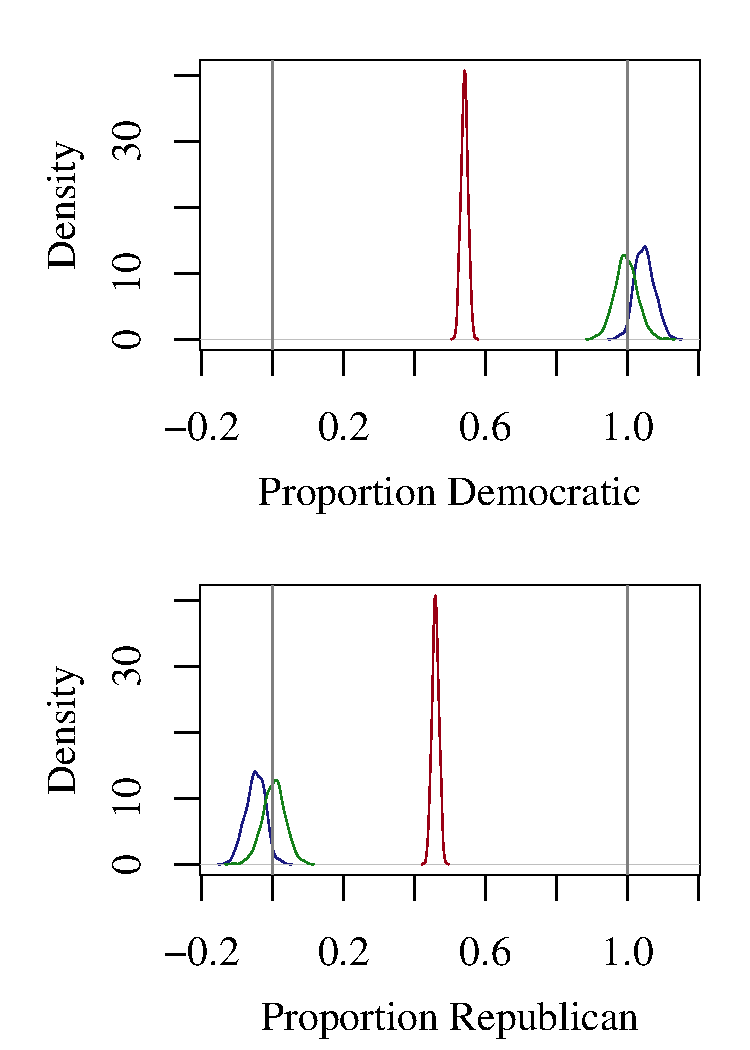
\includegraphics[height=3in]{eiBayesReg.pdf}
\end{center}
\caption{Density plots of Bayesian ecological regression output.}
\label{f:er}
\end{figure}

%\item \begin{verbatim}
%ei.reg(cbind(dem, rep, non) ~ cbind(black, white, natam), 
%   data = senc)
%\end{verbatim}

%\begin{verbatim} 
%lambda.reg(out.reg, columns = c("dem", "rep")) 
%\end{verbatim}
%\item \texttt{density.plot} provides a graphical summary of \texttt{lambda} output:

\subsection{Multinomial-Dirichlet ({\sc md}) model}

In the Multinomial-Dirichlet model \citep{RosJiaKin01}, the
data is expressed as counts and a hierarchical Bayesian model is fit using a
Metropolis-within-Gibbs algorithm implemented in \texttt{C}.  Level 1
models the observed column marginals as Multinomial (and independent
across units); Level 2 models the unobserved rows of cell fraction as
Dirichlet (and independent across rows and units); Level 3 models the
Dirichlet parameters as i.i.d. Gamma.  More formally, without a
covariate, the model is

\begin{eqnarray*}
(N_{\cdot 1i}, \dots, N_{\cdot Ci}) &\stackrel{\indep}{\sim}& {\rm
Multinomial}(N_i, \sum_{r=1}^R \beta_{r1i}X_{ri}, \dots, \sum_{r=1}^R \beta_{rCi}X_{ri}) \\
(\beta_{r1i}, \dots, \beta_{rCi}) &\stackrel{\indep}{\sim}& {\rm Dirichlet}(\alpha_{r1}, \dots, \alpha_{rC})\\
\alpha_{rc} &\stackrel{\rm i.i.d.}{\sim}& {\rm Gamma}(\lambda_1,\lambda_2) 
\end{eqnarray*}

With a unit-level covariate $Z_i$ in the second level, the model becomes
\begin{eqnarray*}
(N_{\cdot 1i}, \dots, N_{\cdot Ci}) &\stackrel{\indep}{\sim}& {\rm
Multinomial}(N_i, \sum_{r=1}^R \beta_{r1i}X_{ri}, \dots, \sum_{r=1}^R \beta_{rCi}X_{ri}) \\
(\beta_{r1i}, \dots, \beta_{rCi}) &\stackrel{\indep}{\sim}& {\rm
Dirichlet}\left(d_r\exp(\gamma_{rc} + \delta_{rc}Z_i), \dots, \right. \\
& & \quad\quad \left. d_r\exp(\gamma_{r(C-1)} +
\delta_{r(C-1)}Z_i), d_r \right) \\
d_r &\stackrel{\rm i.i.d.}{\sim}& {\rm Gamma}(\lambda_1, \lambda_2)  
\end{eqnarray*}

Improper uniform priors are assumed for each $\gamma_{rc}$ and
$\delta_{rc}$. The parameterization of the prior on each $(\beta_{r1i}, \dots,
\beta_{rCi})$ implies that the following log-odds ratio of expected
fractions is linear with respect to the covariate $Z_i$:

\begin{displaymath}
\log\left( \frac{E(\beta_{rci})}{E(\beta_{rCi})} \right) = \gamma_{rc}
+ \delta_{rc} Z_i
\end{displaymath}

Conducting an analysis using the {\sc md} model requires two steps.  First,
\texttt{tuneMD} calibrates the tuning parameters used for
Metropolis-Hastings sampling: 

\begin{verbatim}
> tune.nocov <- tuneMD(cbind(dem, rep, non) ~ cbind(black, white, 
+   natam), data = senc, ntunes = 10, sample = 1000, thin = 1000)
\end{verbatim}

\noindent Second, \texttt{ei.MD.bayes} fits the model by calling
\texttt{C} code to generate MCMC draws:

\begin{verbatim}
> out.nocov <- ei.MD.bayes(cbind(dem, rep, non) ~ cbind(black, white,
+   natam), covariate = NULL, data = senc, lambda1 = 4, lambda2 = 2,
+   tune.list = tune.nocov, ...)
\end{verbatim}

The output of this function can be returned as  \texttt{mcmc} objects
or arrays; in the former case, the standard diagnostic tools for
\texttt{mcmc} objects can be applied directly.   The {\sc md} implementation includes \texttt{lambda} and \texttt{density.plot}
functions, usage for which is analogous to ecological regression:

\begin{verbatim}
> lmd <- lambda.MD(out.nocov, columns = c("dem", "rep"))
> density.plot(lmd)
\end{verbatim}

If the precinct-level parameters are returned or saved,
\texttt{cover.plot} plots the central credible intervals for each
precinct.  The segments represent the 95\% central credible intervals
and their medians for each unit (the true value for each precinct is
the red dot, not included in the standard {\tt cover.plot}).

\begin{verbatim}
> cover.plot(out.nocov, row = "white", column = "dem")
\end{verbatim}
\begin{figure}[h]
\begin{center}
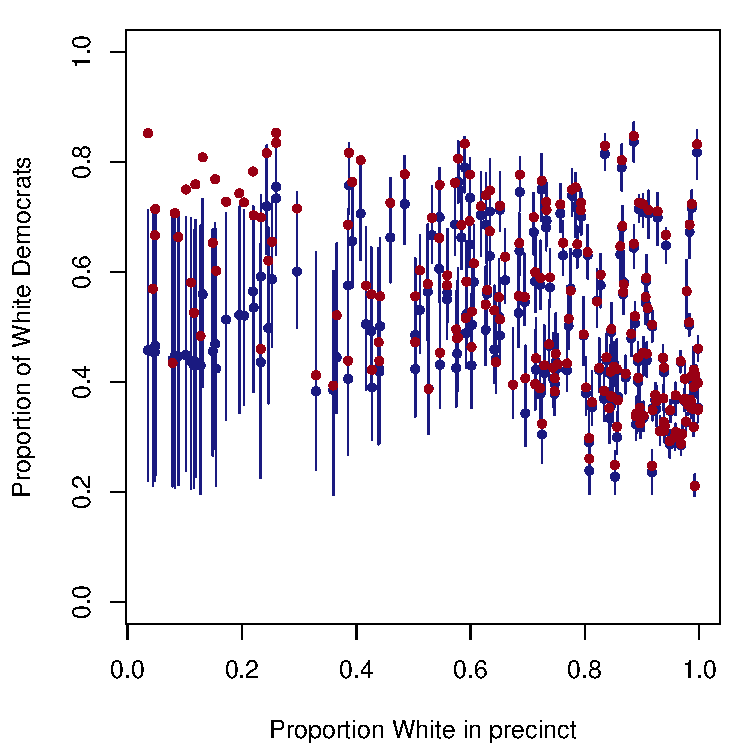
\includegraphics[width=3in]{coversmall.pdf}
\end{center}
\caption{Coverage plot for {\sc md} model output.}
\label{f:md}
\end{figure}
 
%\end{itemize}
%ei.MD.bayes(cbind(dem, rep, non) ~ cbind(black, white, 
%   natam), covariate = NULL, data = senc, lambda1 = 4, 
%   lambda2 = 2,  tune.list = tune.nocov, start.list = NULL, 
%   sample = 1000, thin = 5000, burnin = 1000000, 
%   ret.beta = 'r', ret.mcmc = TRUE, usrfun = NULL)

%cover.plot(out.nocov, row = "white", column = "dem")


\section{Data Management}

In the {\sc md} model, reasonable-sized problems produce unreasonable
amounts of data.  For example, a model for voting in Ohio includes
11000 precincts, 3 racial groups, and 4 parties.  Implementing 1000
iterations yields about 130 million parameter draws.  These draws
occupy about 1GB of RAM, and this is almost certainly not enough
iterations.  We provide a few options to users in order to make this
model tractable for large {\sc ei} problems. 


The unit-level parameters present the most significant data management
problem.  Rather than storing unit-level parameters in the workspace, users can
save each chain as a {\tt .tar.gz} file on disk using the option
\texttt{ei.MD.bayes(..., ret.beta = "s")}, or discard the unit-level
draws entirely using \texttt{ei.MD.bayes(..., ret.beta = "d")}.  To
reconstruct the chains, users can select the row marginals, column
marginals, and units of interest, without reconstructing the entire
matrix of unit-level draws:   

\begin{verbatim}
> read.betas(rows = c("black", "white"), columns = c("dem"), 
+   units = 1:150, dir = getwd())
\end{verbatim}

If users are interested in some function of the unit-level parameters,
the implementation of the {\sc md} model allows them to define a
function in \texttt{R} that will be called from within the \texttt{C}
sampling algorithm, in which case the unit-level parameters need not
be saved for post-processing.

\section{Conclusion}

\texttt{eiPack} was developed with the support of the Institute for
Quantitative Social Science at Harvard University.  Thanks to Gary King, Kevin Quinn, and D. James Greiner for
suggestions and Matt Cox and Bob Kinney for technical advice.
For further information, see \\
\texttt{http://www.people.fas.harvard.edu/$\sim$olau/software/eiPack.html}.

 

\bibliographystyle{apsr}
\bibliography{ei}


\end{document}
